\section{Conclusion and Future Work}
We present a compact representation of PRT for \textbf{free form} deformable objects, informing of a non-linear model, namely a deep convolutional neural network, with significant memory savings demonstrated.
 The model is able to extract the features of the dataset relevant to the light transfer function and thus generate good visual approximations for a wide spectrum of deformations, with resulting appearances that are practically indistinguishable from the ground truth.  

Moreover, our method shows much higher generalization properties than previous approaches, allowing deformations from much larger and less constrained deformation spaces.

Although we showed DeepPRT can be much more compact than traditional PRT, our network is far from being optimal. Exploiting network compression and acceleration methods could be highly beneficial \cite{Survey_NN_Compression, Deep_Compression}.
Moreover, other network topologies and/or cost functions could be explored in order to achieve better approximations, for instance, as proposed in \cite{Deformable_UNet} to account for individual object deformations the use of deformable convolutions \cite{DeformableCNN} could be investigated. Further to the transfer function representation, a direct learning of more bespoke and compact representations \cite{Sloan2018} could also be applied in this context.

The particular choice of our basis functions (Spherical Harmonics), currently restricts our method to low-frequency lightings. However, an extension to all-frequencies is possible by fitting the model to an alternative representation of the transfer function $T$, such as non-linear Wavelets \cite{AllFrequencyPRT}.

The most significant further area of interest for our method resides within the choice of our parametrization (harmonic map). Harmonic mapping performs well for modest curvature variations and is restricted to surfaces with one boundary (topological disks); however, using the geometric-stretch parametrization instead and further using the extension proposed by \cite{Spherical_Parametrization}, the representation would be more accurate in reconstruction of shape. The U-Net process in this context of sharp feature reconstruction and non-disk topologies would need additional measures. In particular, a treatment of the \textit{diffeomorphic} behavior \cite{detlefsen2018transformations} of these mappings appropriate to efficient deep learning of light transport for animating arbitrary surfaces would be interesting to further understand the representation trade-offs.
%%%%%%%%%%%%%%%%%%%%%%%%%%%%% 
%\textit{\begin{figure*}
%  \centering
%    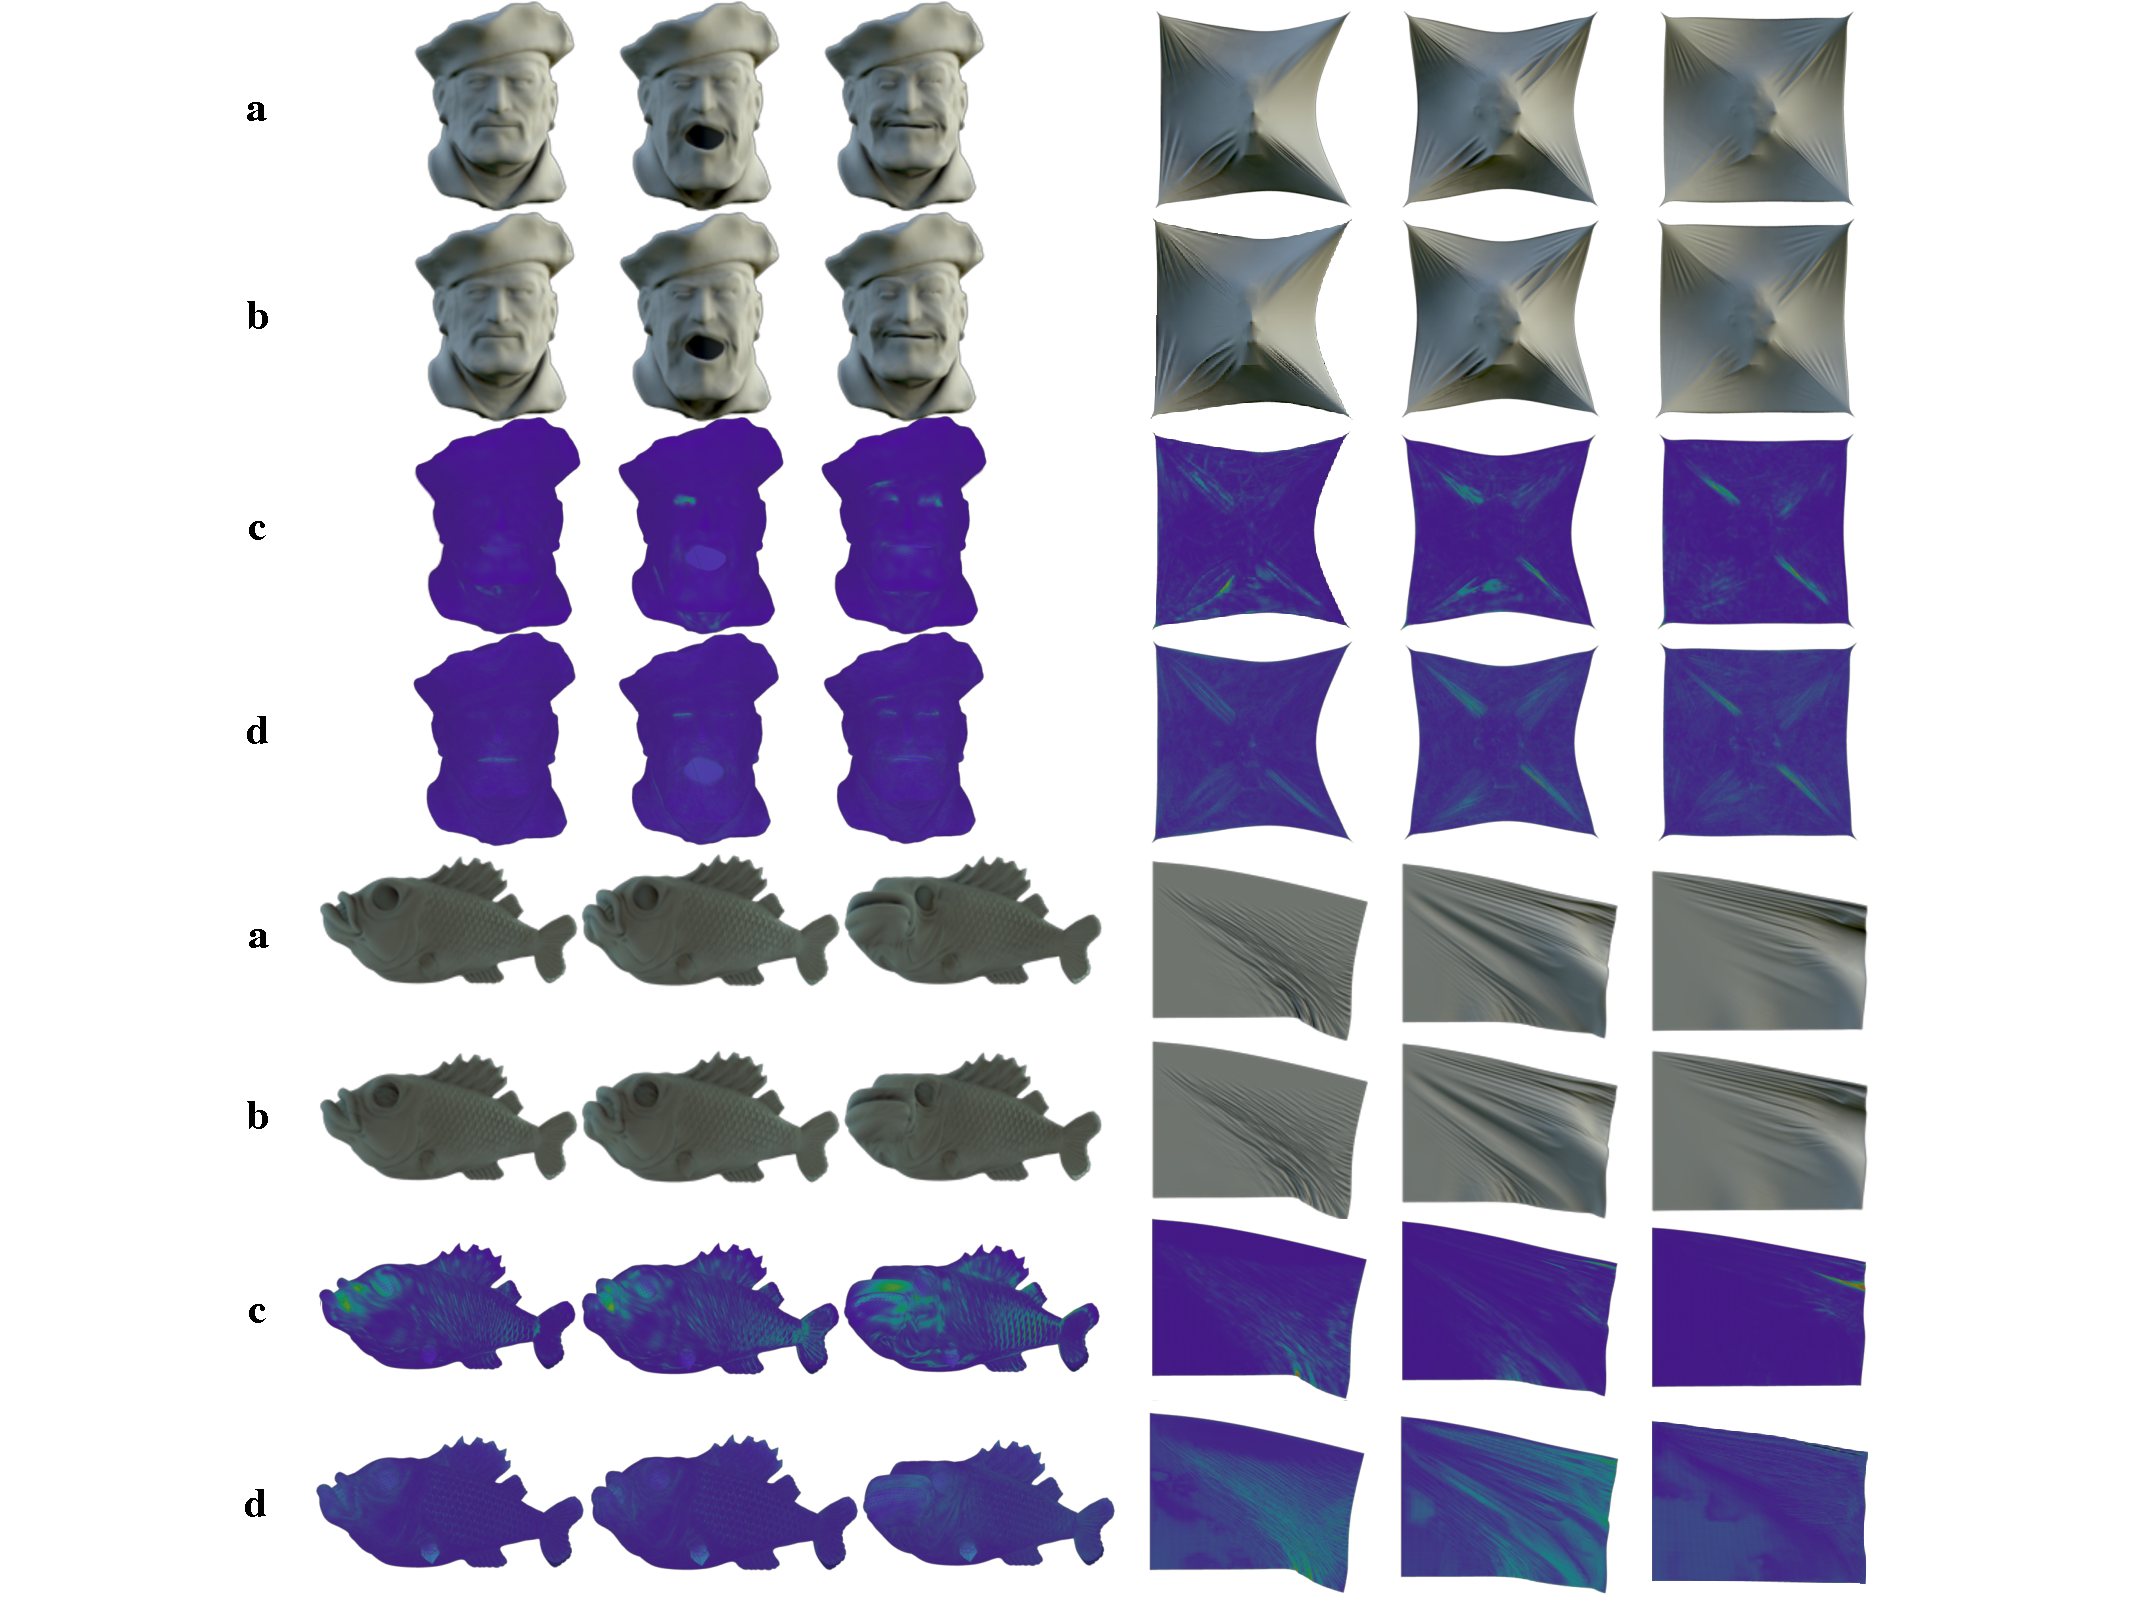
\includegraphics[width=0.5\paperwidth]{Figures/DPRT_quality_SSIM.pdf}
%     \caption{Prediction Quality:
%     a : ground truth appearance. b: predicted appearance. c: SSIM. d: L1-Error between ground truth and predicted transfer coefficients }
%     \label{Fig: DPRT_Quality}
%\end{figure*}}
\begin{figure}[H]
  \centering
    \includegraphics[height=\textheight]{Figures/DPRT_quality_SSIM_vert.pdf}
     \caption{Prediction Quality:
     a) ground truth appearance. b) predicted appearance. c) SSIM. d) L1-Error between ground truth and predicted transfer coefficients }
     \label{Fig: DPRT_Quality}
\end{figure}

\begin{acks}
omitted
\end{acks}